\documentclass[12pt,a4paper]{article}

% --- Paquetes ---
\usepackage[utf8]{inputenc}
\usepackage[spanish]{babel}
\usepackage[margin=2.5cm]{geometry}
\usepackage{graphicx}
\usepackage{hyperref}
\usepackage{titlesec}
\usepackage{listings}
\usepackage{xcolor}
\usepackage{float}
\usepackage{booktabs}

% --- Configuración de Colores para Métricas ---
\definecolor{metGood}{rgb}{0.0, 0.6, 0.0}
\definecolor{metMedium}{rgb}{1.0, 0.5, 0.0}
\definecolor{metBad}{rgb}{0.8, 0.0, 0.0}
\newcommand{\good}[1]{\textbf{\textcolor{metGood}{#1}}}
\newcommand{\medium}[1]{\textbf{\textcolor{metMedium}{#1}}}
\newcommand{\bad}[1]{\textbf{\textcolor{metBad}{#1}}}

% --- Configuración de Estilo ---
\hypersetup{
  colorlinks=true,
  linkcolor=blue,
  filecolor=magenta,
  urlcolor=cyan,
}

\definecolor{uahblue}{rgb}{0.0, 0.27, 0.55}

\begin{document}

\begin{titlepage}
    \centering

    % --- Cabecera ---
    {\large\color{uahblue}\textbf{Universidad de Alcalá}}\\[0.3em]
    {\normalsize Escuela Politécnica Superior}\\[0.2em]
    {\normalsize Calidad y Pruebas del Software}

    \vspace{1.5cm}
    {\color{uahblue}\rule{\linewidth}{1.5pt}}
    \vspace{0.5cm}

    % --- Título ---
    {\Huge\bfseries Práctica 2}\\[0.6em]
    {\LARGE Calidad, Fiabilidad y Mantenimiento}

    \vspace{0.5cm}
    {\color{uahblue}\rule{\linewidth}{1.5pt}}
    \vspace{2cm}

    % --- Autores ---
    {\large
        \begin{tabular}{c}
            Daniel Apellido1 Apellido2   \\[0.4em]
            Nacho Apellido1 Apellido2    \\[0.4em]
            Jaime Apellido1 Apellido2    \\
        \end{tabular}
    }

    \vfill

    % --- Fecha ---
    {\large\today}

\end{titlepage}
\newpage

\tableofcontents
\newpage

\section{Parte 1: Herramientas de medida de software}
En esta sección se analiza el proyecto utilizando la herramienta \texttt{Radon} para extraer métricas de software relevantes.

\subsection{Análisis de métricas (Radon)}

% --- Tabla 1: Complejidad Ciclomática ---
\begin{table}[H]
    \centering
    \footnotesize
    \setlength{\tabcolsep}{4pt}
    \begin{tabular}{lccl cc}
        \toprule
        \textbf{Fichero}                       & \textbf{Tipo} & \textbf{Línea} & \textbf{Nombre}               & \textbf{CC} & \textbf{Grado} \\
        \midrule
        texttest\_fixture.py                   & F             & 7:0            & main                          & 4           & \good{A}       \\
        gilded\_rose.py                        & M             & 8:4            & GildedRose.update\_quality    & 19          & \medium{C}     \\
        gilded\_rose.py                        & C             & 3:0            & GildedRose                    & 11          & \medium{C}     \\
        gilded\_rose.py                        & C             & 39:0           & Item                          & 2           & \good{A}       \\
        gilded\_rose.py                        & M             & 5:4            & GildedRose.\_\_init\_\_       & 1           & \good{A}       \\
        gilded\_rose.py                        & M             & 40:4           & Item.\_\_init\_\_             & 1           & \good{A}       \\
        gilded\_rose.py                        & M             & 45:4           & Item.\_\_repr\_\_             & 1           & \good{A}       \\
        src/python/\_\_init\_\_.py             & F             & 1:0            & hello                         & 1           & \good{A}       \\
        tests/test\_gilded\_rose\_approvals.py & F             & 7:0            & test\_gilded\_rose\_approvals & 1           & \good{A}       \\
        \bottomrule
    \end{tabular}
    \caption{Resultados de Complejidad Ciclomática (Radon CC)}
    \label{tab:radon_cc}
\end{table}

% --- Tabla 2: Métricas Raw ---
\begin{table}[H]
    \centering
    \small
    \begin{tabular}{lccccc}
        \toprule
        \textbf{Fichero}                       & \textbf{LOC} & \textbf{LLOC} & \textbf{SLOC} & \textbf{Coment.} & \textbf{Blank} \\
        \midrule
        texttest\_fixture.py                   & 36           & 22            & 29            & 2                & 6              \\
        gilded\_rose.py                        & 46           & 39            & 39            & 1                & 6              \\
        src/python/\_\_init\_\_.py             & 2            & 2             & 2             & 0                & 0              \\
        tests/test\_gilded\_rose\_approvals.py & 21           & 17            & 17            & 0                & 4              \\
        tests/test\_gilded\_rose.py            & 16           & 10            & 10            & 1                & 5              \\
        tests/\_\_init\_\_.py                  & 0            & 0             & 0             & 0                & 0              \\
        tests/conftest.py                      & 0            & 0             & 0             & 0                & 0              \\
        \bottomrule
    \end{tabular}
    \caption{Métricas Raw (Radon RAW)}
    \label{tab:radon_raw}
\end{table}

% --- Tabla 3: Métricas de Halstead ---
\begin{table}[H]
    \centering
    \small
    \setlength{\tabcolsep}{4pt}
    \begin{tabular}{lcccccccc c}
        \toprule
        \textbf{Fichero}            & \textbf{$n_1$} & \textbf{$n_2$} & \textbf{$N_1$} & \textbf{$N_2$} & \textbf{Vocab.} & \textbf{Vol.} & \textbf{Diff.} & \textbf{Effort} & \textbf{Bugs}  \\
        \midrule
        texttest\_fixture.py        & 5              & 12             & 9              & 17             & 17              & 106.27        & 3.54           & 376.39          & \good{0.035}   \\
        gilded\_rose.py             & 8              & 15             & 27             & 54             & 23              & 366.41        & 14.40          & \bad{5276.28}   & \medium{0.122} \\
        tests/.../approvals.py      & 1              & 2              & 1              & 2              & 3               & 4.75          & 0.50           & 2.38            & \good{0.002}   \\
        tests/test\_gilded\_rose.py & 1              & 2              & 1              & 2              & 3               & 4.75          & 0.50           & 2.38            & \good{0.002}   \\
        src/python/\_\_init\_\_.py  & 0              & 0              & 0              & 0              & 0               & 0.00          & 0.00           & 0.00            & \good{0.000}   \\
        tests/\_\_init\_\_.py       & 0              & 0              & 0              & 0              & 0               & 0.00          & 0.00           & 0.00            & \good{0.000}   \\
        tests/conftest.py           & 0              & 0              & 0              & 0              & 0               & 0.00          & 0.00           & 0.00            & \good{0.000}   \\
        \bottomrule
    \end{tabular}
    \caption{Métricas de Halstead (Radon HAL)}
    \label{tab:radon_hal}
\end{table}

% --- Tabla 4: Maintainability Index ---
\begin{table}[H]
    \centering
    \small
    \begin{tabular}{lcc}
        \toprule
        \textbf{Fichero}                       & \textbf{Score} & \textbf{Grado} \\
        \midrule
        texttest\_fixture.py                   & 70.99          & \good{A}       \\
        gilded\_rose.py                        & 53.77          & \good{A}       \\
        src/python/\_\_init\_\_.py             & 100.00         & \good{A}       \\
        tests/test\_gilded\_rose\_approvals.py & 68.15          & \good{A}       \\
        tests/test\_gilded\_rose.py            & 61.88          & \good{A}       \\
        tests/\_\_init\_\_.py                  & 100.00         & \good{A}       \\
        tests/conftest.py                      & 100.00         & \good{A}       \\
        \bottomrule
    \end{tabular}
    \caption{Maintainability Index (Radon MI)}
    \label{tab:radon_mi}
\end{table}

\subsection{Interpretación y Justificación}
Antes de proceder con la comparativa, es fundamental entender qué mide cada una de las métricas extraídas:

\begin{itemize}
    \item \textbf{Complejidad Ciclomática (CC):} Mide el número de caminos linealmente
          independientes a través del código, el cual aumenta con el número de bifurcaciones.
          Una complejidad alta indica una lógica de control difícil de seguir y testear.
          Por ejemplo, el número de casos de prueba necesario para cubrir
          completamente el código aumenta exponencialmente con la complejidad.
    \item \textbf{Métricas Raw (RAW):} Proporcionan conteos básicos que permiten evaluar
          el tamaño físico del software y cuán documentado está el código:
          \textbf{LOC} (\textit{Lines of Code}) cuenta el total de líneas del fichero;
          \textbf{LLOC} (\textit{Logical Lines of Code}) cuenta las instrucciones lógicas
          (asignaciones, condicionales, llamadas, etc.);
          \textbf{SLOC} (\textit{Source Lines of Code}) cuenta únicamente las líneas con código
          real, excluyendo comentarios y líneas en blanco, siendo el indicador más representativo
          del tamaño efectivo;
          \textbf{Coment.} recoge las líneas de comentario, cuya proporción respecto a SLOC es un
          indicador directo de documentación y, por ende, de mantenibilidad;
          y \textbf{Blank} contabiliza las líneas en blanco, que influyen en la legibilidad.
    \item \textbf{Métricas de Halstead (HAL):} Evalúan la complejidad algorítmica basándose en el
          número de operadores y operandos únicos usados ($n_1, n_2$) y el número de operadores y
          operandos totales sin unicidad ($N_1, N_2$). Incluye el \textit{Vocabulario} (número de
          operadores y operandos únicos), el \textit{Volumen} (tamaño de la implementación) y
          el \textit{Esfuerzo} (carga mental para entender el código). Además, estima la probabilidad
          de errores (Bugs) basándose en el volumen y el vocabulario.
          Un esfuerzo alto indica que el código es difícil de entender y mantener, lo que puede
          traducirse en una mayor probabilidad de introducir errores en futuras modificaciones.
    \item \textbf{Índice de Mantenibilidad (MI):} Un valor compuesto que estima la
          facilidad con la que el software puede ser mantenido, combinando CC, Halstead y
          el tamaño del código. A mayor valor, mejor mantenibilidad. Sin embargo, es
          importante destacar que el MI puede ser engañoso en archivos pequeños, ya que
          tiende a ser artificialmente alto en este caso.
\end{itemize}

Al realizar un análisis comparativo entre los distintos módulos del proyecto, se observa
una clara disparidad en la calidad del código, concentrándose la mayor deuda técnica en el
archivo \texttt{gilded\_rose.py}.

\begin{itemize}
    \item \textbf{Comparativa de Complejidad (CC):} Mientras que los módulos de apoyo
          como \texttt{texttest\_fixture.py} y los tests mantienen una complejidad de grado
          \good{A} (valores entre 1 y 5), el archivo \texttt{gilded\_rose.py} destaca
          negativamente con un grado \medium{C} (valores entre 11 y 20) en su método
          principal. Esta diferencia subraya que en el archivo \texttt{gilded\_rose.py},
          en específico en el método \texttt{update\_quality}, la lógica de control es
          mucho más intrincada debido a un mayor número de bifurcaciones, lo que
          dificulta su comprensión y mantenimiento.

    \item \textbf{Distribución del Esfuerzo (Halstead):} El contraste en el esfuerzo mental
          (Effort) es el más revelador. El archivo \texttt{gilded\_rose.py} registra un valor de
          \bad{5276.28}, lo que supone casi 14 veces más esfuerzo que el siguiente archivo más complejo
          (\texttt{texttest\_fixture.py} con 376.39) y miles de veces más que los archivos de test.
          Esto posiciona a \texttt{gilded\_rose.py} como el cuello de botella crítico para cualquier
          mantenimiento futuro.

    \item \textbf{Densidad de Errores y Tamaño:} A pesar de que todos los archivos tienen un tamaño
          similar en líneas de código (RAW), con \texttt{gilded\_rose.py} (39 SLOC) y
          \texttt{texttest\_fixture.py} (29 SLOC) muy parejos, la probabilidad de bugs estimada por
          Halstead es notablemente superior en el primero (\medium{0.122} frente a \good{0.035}). Esto
          confirma que no es el tamaño del archivo lo que genera el riesgo, sino la densidad de
          operaciones y operandos.

    \item \textbf{Limitaciones del Índice de Mantenibilidad (MI):} Curiosamente, todos
          los archivos presentan un grado \good{A} en el índice MI. Sin embargo, al compararlo
          con el esfuerzo de Halstead, se hace evidente que el MI tiende a ser optimista en
          archivos pequeños, ocultando la complejidad real que sí detectan las métricas de CC y Effort.
\end{itemize}

\newpage
\section{Parte 2: Fiabilidad del sistema}
Análisis del comportamiento de la aplicación desde el punto de vista de la fiabilidad, simulando un entorno de servidor propenso a fallos.

\subsection{Implementación de la herramienta de cálculo}
\textit{Resumen de cómo se ha implementado el archivo Excel para el cálculo automático de indicadores básico de fiabilidad.}

\subsection{Indicadores de Fiabilidad}
\textit{Documentar los indicadores calculados: número de fallos, MTBF, MTTF, MTTR, disponibilidad, etc.}

\subsection{Representación Gráfica y Curva de Fiabilidad}
\textit{Incluir gráficas desarrolladas de los periodos de funcionamiento y fallo, así como la curva de fiabilidad $R(t) = e^{-\lambda \cdot t}$.}

\newpage
\section{Parte 3: Mantenimiento y mejora de calidad}
Propuesta y ejecución de mejoras en el código para optimizar el diseño y mejorar las métricas obtenidas anteriormente.

Lo primero que se ha realizado es un conjunto de tests a partir de la funcionalidad indicada en los requisitos de Gilded Rose, para posteriormente realizar una refactorización del código y mejorar las métricas obtenidas en la Parte 1. De esta manera, podemos asegurar el correcto funcionamiento del código mientras es refactorizado.

\subsection{Tests desarrollados}

A continuación se muestran los tests desarrollados para cada uno de los tipos de ítems del sistema, así como los tests de invariantes globales (calidad nunca negativa ni superior a 50):

\begin{figure}[H]
    \centering
    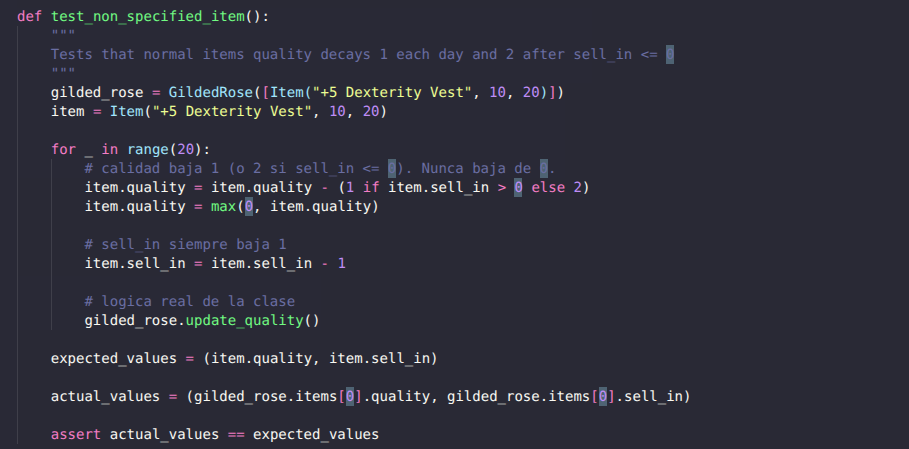
\includegraphics[width=\textwidth]{imgs/test_non_specified.png}
    \caption{Test: ítems sin categoría especial}
    \label{fig:test_non_specified}
\end{figure}

\begin{figure}[H]
    \centering
    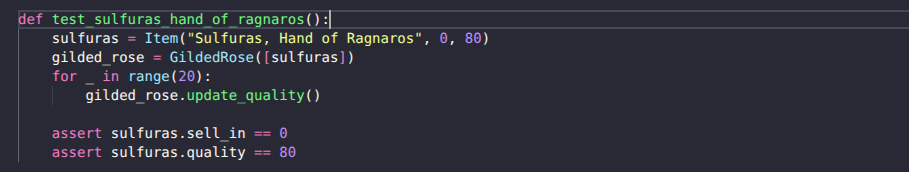
\includegraphics[width=\textwidth]{imgs/test_sulfuras.png}
    \caption{Test: Sulfuras, Hand of Ragnaros}
    \label{fig:test_sulfuras}
\end{figure}

\begin{figure}[H]
    \centering
    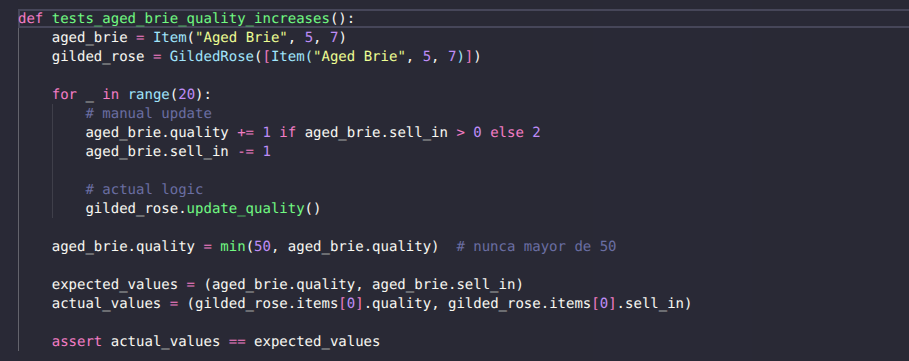
\includegraphics[width=\textwidth]{imgs/test_aged_brie.png}
    \caption{Test: Aged Brie}
    \label{fig:test_aged_brie}
\end{figure}

\begin{figure}[H]
    \centering
    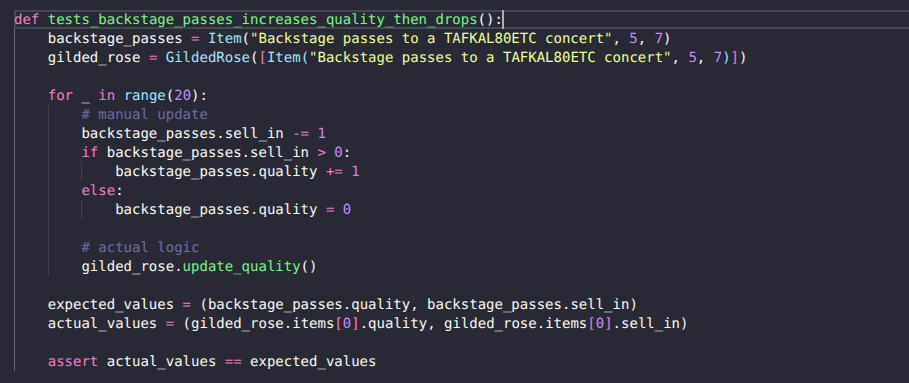
\includegraphics[width=\textwidth]{imgs/test_backstage_passes.png}
    \caption{Test: Backstage passes}
    \label{fig:test_backstage_passes}
\end{figure}

\begin{figure}[H]
    \centering
    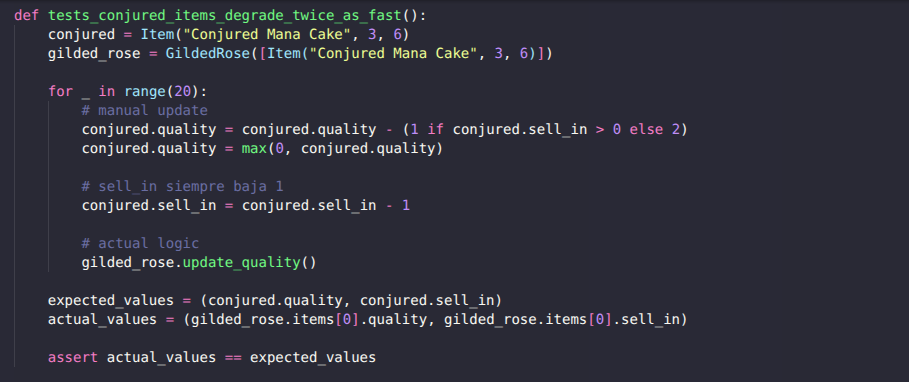
\includegraphics[width=\textwidth]{imgs/test_conjured.png}
    \caption{Test: Conjured Mana Cake}
    \label{fig:test_conjured}
\end{figure}

\begin{figure}[H]
    \centering
    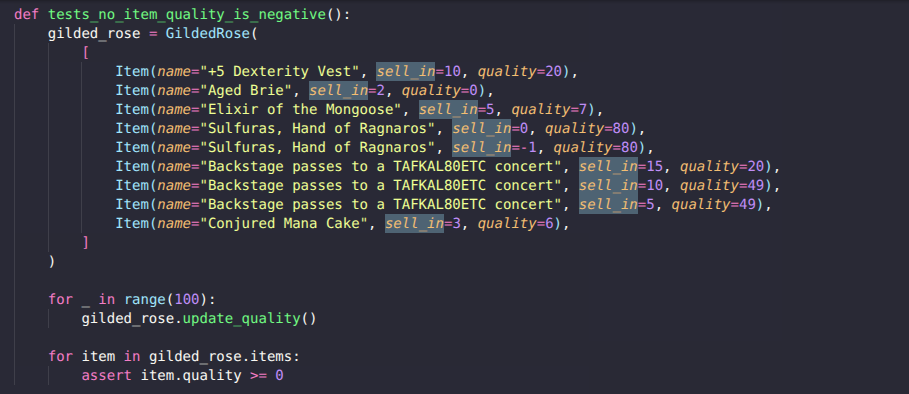
\includegraphics[width=\textwidth]{imgs/test_no_negative_qualities.png}
    \caption{Test: la calidad nunca es negativa}
    \label{fig:test_no_negative_qualities}
\end{figure}

\begin{figure}[H]
    \centering
    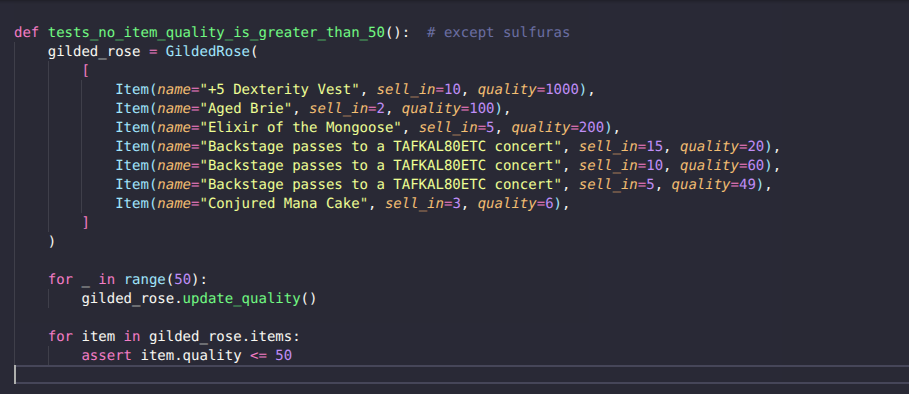
\includegraphics[width=\textwidth]{imgs/test_no_greater_50.png}
    \caption{Test: la calidad nunca supera 50}
    \label{fig:test_no_greater_50}
\end{figure}

\subsection{Análisis de mejoras propuestas}

A partir de los tests desarrollados y del análisis de métricas de la Parte 1, se identifican las siguientes mejoras:

\begin{itemize}
    \item \textbf{Separación de lógica por tipo de ítem:} Analizar y encapsular la lógica para cada
          tipo de objeto (Aged Brie, Sulfuras, Backstage Passes y cualquier otro) de forma
          independiente, facilitando la lectura y la comprensión de cada caso.
    \item \textbf{Sustitución de bifurcaciones por operaciones matemáticas:} Reemplazar la lógica
          de limitación de calidad ($0 \leq \mathrm{calidad} \leq 50$) por el uso de \texttt{max} y
          \texttt{min}, reduciendo el número de ramas y, por tanto, la complejidad ciclomática.
    \item \textbf{Generalización del flujo común:} Introducir en el flujo de control general las
          modificaciones que se aplican a todos los objetos (o a la mayoría), dejando las excepciones
          como casos particulares.
    \item \textbf{Documentación del código:} Añadir comentarios explicativos en cada bloque lógico
          para facilitar su comprensión y, por ende, su mantenibilidad futura.
    \item \textbf{Eliminación de código duplicado:} Simplificar la lógica de cada tipo de ítem
          suprimiendo redundancias y mejorando la claridad del flujo.
\end{itemize}

\subsection{Cambios realizados en el código}

Aplicando las mejoras anteriores, el código refactorizado resultante es el siguiente:

\begin{figure}[H]
    \centering
    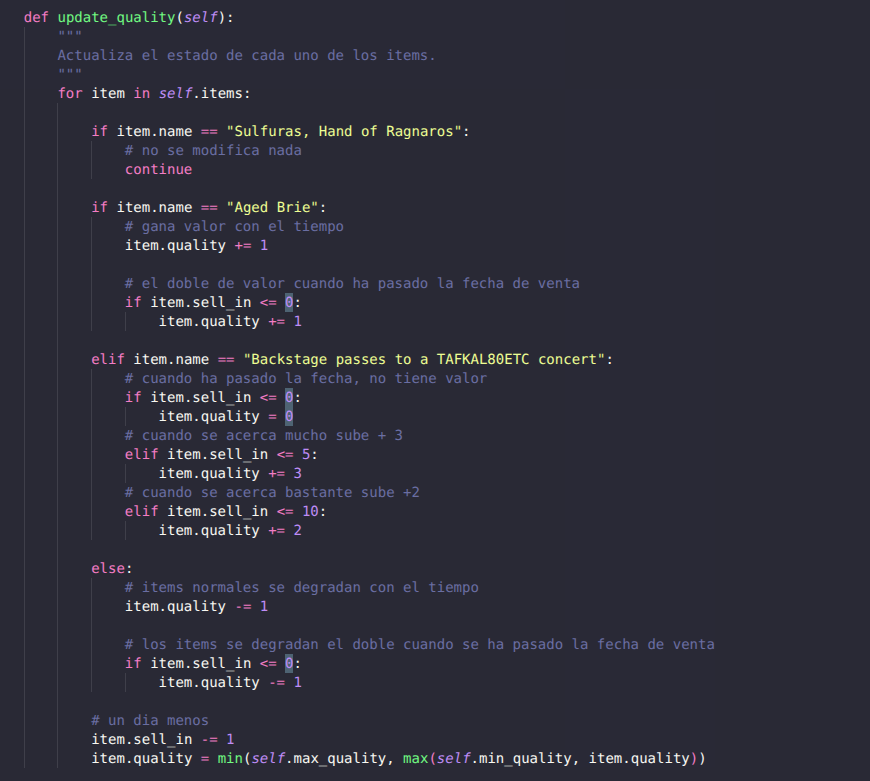
\includegraphics[width=\textwidth]{imgs/gilded_refactor.png}
    \caption{Código refactorizado de \texttt{gilded\_rose.py}}
    \label{fig:refactored_code}
\end{figure}

No obstante, estas mejoras se realizan respetando las restricciones indicadas en los requisitos originales. Si se quisiera una mayor mantenibilidad y seguir más estrictamente el principio de responsabilidad única, se podría definir un conjunto de comportamientos asignados a los objetos mediante composición. En otras palabras, se podría aplicar el \textit{Strategy Pattern} para encapsular el comportamiento de cada tipo de ítem de forma intercambiable.

\subsection{Comparativa de resultados}

Las siguientes tablas comparan las métricas de \texttt{gilded\_rose.py} antes y después de la refactorización.

\begin{table}[H]
    \centering
    \small
    \begin{tabular}{lccc c}
        \toprule
        \textbf{Nombre}            & \textbf{Tipo} & \textbf{Grado anterior} & \textbf{Grado actual} & \textbf{Mejora} \\
        \midrule
        GildedRose.update\_quality & M             & \medium{C} (19)         & \medium{B} (10)       & $\uparrow$      \\
        GildedRose                 & C             & \medium{C} (11)         & \medium{B} (7)        & $\uparrow$      \\
        \bottomrule
    \end{tabular}
    \caption{Comparativa de Complejidad Ciclomática (Radon CC)}
    \label{tab:cc_comparativa}
\end{table}

\begin{table}[H]
    \centering
    \small
    \begin{tabular}{lccccc}
        \toprule
        \textbf{Métrica} & \textbf{LOC} & \textbf{LLOC} & \textbf{SLOC} & \textbf{Coment.} & \textbf{Blank} \\
        \midrule
        Antes            & 46           & 39            & 39            & 1                & 6              \\
        Después          & 76           & 38            & 33            & 9                & 13             \\
        \bottomrule
    \end{tabular}
    \caption{Comparativa de Métricas Raw (Radon RAW)}
    \label{tab:raw_comparativa}
\end{table}

\begin{table}[H]
    \centering
    \small
    \setlength{\tabcolsep}{4pt}
    \begin{tabular}{lcccccccc c}
        \toprule
        \textbf{Estado} & \textbf{$n_1$} & \textbf{$n_2$} & \textbf{$N_1$} & \textbf{$N_2$} & \textbf{Vocab.} & \textbf{Vol.} & \textbf{Diff.} & \textbf{Effort}  & \textbf{Bugs}  \\
        \midrule
        Antes           & 8              & 15             & 27             & 54             & 23              & 366.41        & 14.40          & \bad{5276.28}    & \medium{0.122} \\
        Después         & 5              & 14             & 16             & 32             & 19              & 203.90        & 5.71           & \medium{1165.15} & \good{0.068}   \\
        \bottomrule
    \end{tabular}
    \caption{Comparativa de Métricas de Halstead (Radon HAL)}
    \label{tab:hal_comparativa}
\end{table}

\begin{table}[H]
    \centering
    \small
    \begin{tabular}{lcc}
        \toprule
        \textbf{Estado} & \textbf{Score} & \textbf{Grado} \\
        \midrule
        Antes           & 53.77          & \good{A}       \\
        Después         & 74.36          & \good{A}       \\
        \bottomrule
    \end{tabular}
    \caption{Comparativa de Maintainability Index (Radon MI)}
    \label{tab:mi_comparativa}
\end{table}

La refactorización produce mejoras en todas las métricas relevantes. En CC, tanto \texttt{update\_quality} como la clase \texttt{GildedRose} reducen su grado de \medium{C} a \medium{B}, gracias a la separación de la lógica en bloques independientes por tipo de ítem. En Halstead, el esfuerzo cae de \bad{5276.28} a \medium{1165.15} (una reducción del 78\%), y la probabilidad de bugs estimada mejora de \medium{0.122} a \good{0.068}. En Raw, el SLOC efectivo se reduce de 39 a 33 líneas, mientras que los comentarios pasan de 1 a 9, reflejando la mayor documentación introducida. El MI mejora de 53.77 a 74.36, manteniéndose en grado \good{A} y confirmando que la refactorización ha mejorado la mantenibilidad global.

\end{document}
